\begin{figure}[h!]
   \centering
   \begin{subfigure}[b]{0.6\textwidth}
      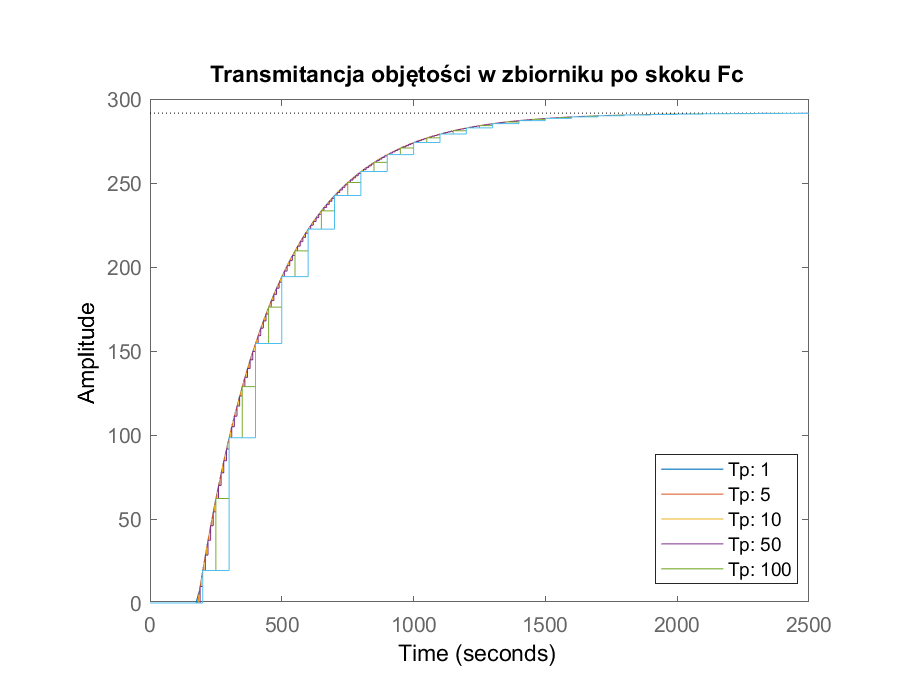
\includegraphics[width=1\linewidth]{img/transforms/transformVFc.eps}
      \caption{}
      \label{fig:fig:transformV1}
   \end{subfigure}
       
   \begin{subfigure}[b]{0.6\textwidth}
      \includegraphics[width=1\linewidth]{img/transforms/transformVFh.eps}
      \caption{}
      \label{fig:fig:transformV2}
   \end{subfigure}
       
   \begin{subfigure}[b]{0.6\textwidth}
      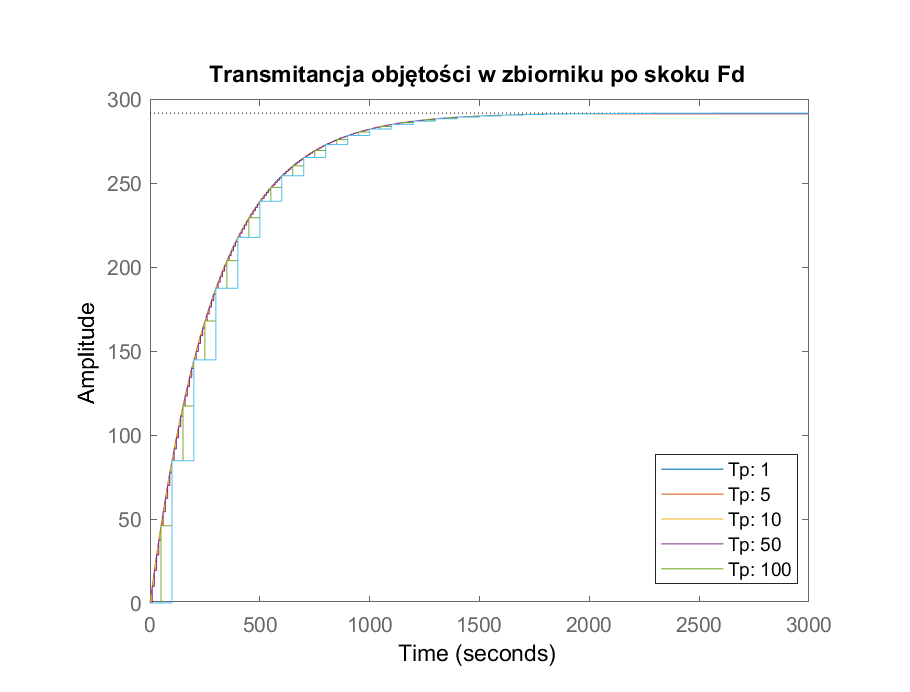
\includegraphics[width=1\linewidth]{img/transforms/transformVFd.eps}
      \caption{}
      \label{fig:fig:transformV3}
   \end{subfigure}
       
   \caption{Wykresy dla transmitancji objętości}
   \label{fig:transformV}
\end{figure}
           
\begin{figure}[h!]
   \centering
   \begin{subfigure}[b]{0.6\textwidth}
      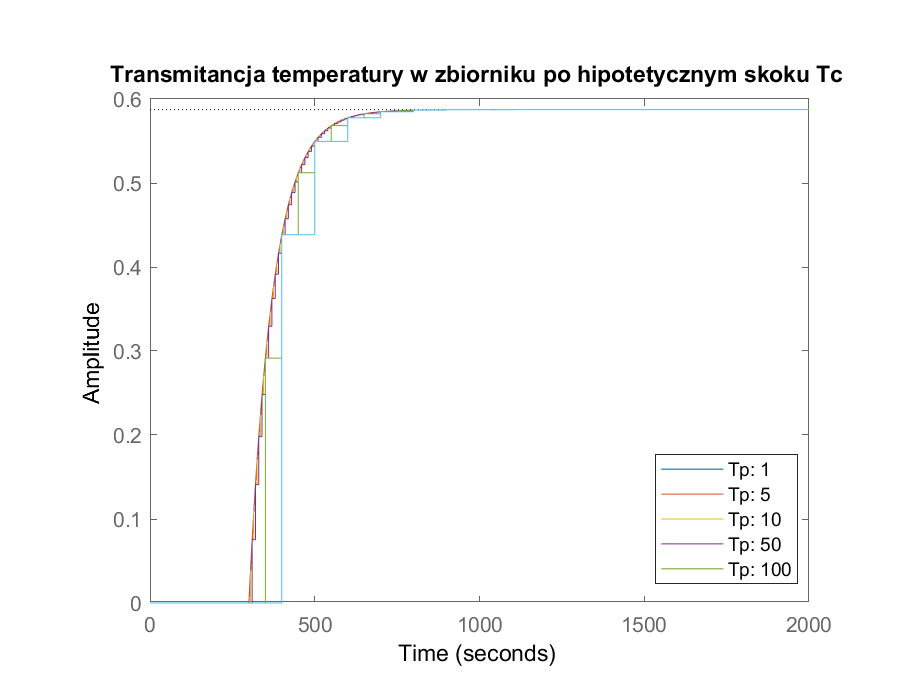
\includegraphics[width=1\linewidth]{img/transforms/transformTTc.eps}
      \caption{}
      \label{fig:fig:transformTT1}
   \end{subfigure}
       
   \begin{subfigure}[b]{0.6\textwidth}
      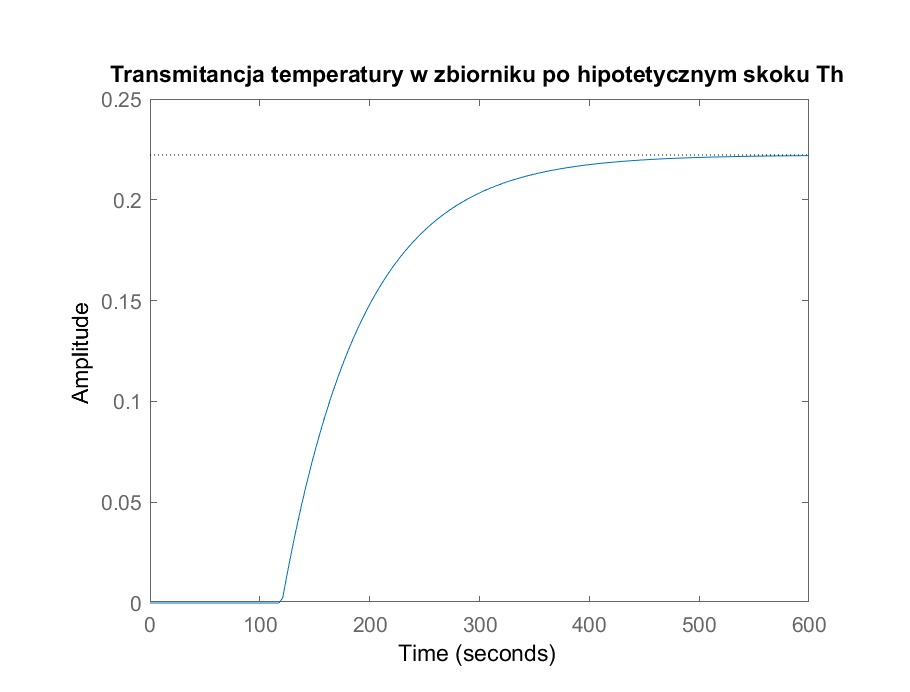
\includegraphics[width=1\linewidth]{img/transforms/transformTTh.eps}
      \caption{}
      \label{fig:fig:transformTT2}
   \end{subfigure}
       
   \begin{subfigure}[b]{0.6\textwidth}
      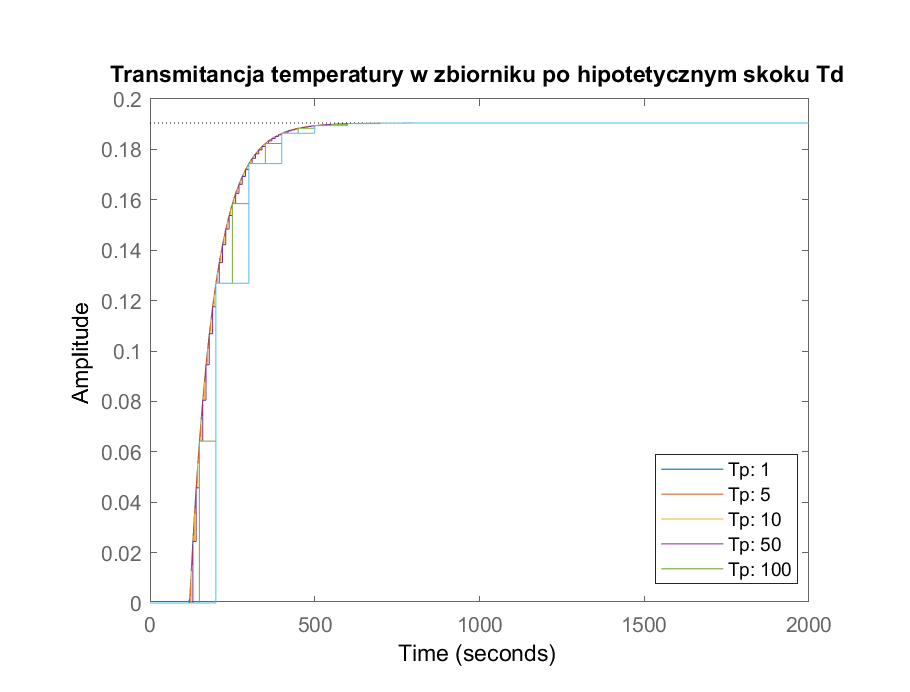
\includegraphics[width=1\linewidth]{img/transforms/transformTTd.eps}
      \caption{}
      \label{fig:fig:transformTT3}
   \end{subfigure}
       
   \caption{Wykresy dla transmitancji temperatury wyjściowej po zmianie temperatury cieczy}
   \label{fig:transformTT}
\end{figure}
           
